% !TeX spellcheck = en_US
%Publications.tex
%\newcommand{\PublicationsPath}{PatentsAndPublications/Publications}

%BMSB2020

\section[Adaptive Rate Control for Live streaming using SRT protocol]{Adaptive Rate Control for Live streaming using SRT protocol}
\label{chap:BMSB2020}
\begin{itemize} \itemsep1pt\parskip0pt\parsep0pt
	\item \textbf{Title:} Adaptive Rate Control for Live streaming using SRT protocol
	\item \textbf{Authors:} Roberto Viola, \'Angel Mart\'in, Juan Felipe Mogoll\'on, Alvaro Gabilondo, Javier Morgade and Mikel Zorrilla
	\item \textbf{Proceedings:} 2020 IEEE International Symposium on Broadband Multimedia Systems and Broadcasting (BMSB)
	\item \textbf{Publisher:} IEEE
	\item \textbf{Year:} 2020
	\item \textbf{DOI:}  \url{10.1109/BMSB49480.2020.9379708}
\end{itemize}

\textbf{Abstract:} Media delivery represents one of the main challenges for future networks which aim to converge Broadcast and Broadband video traffic into a common telecommunication network architecture. Nowadays, contents streamed over Internet are delivered in two different manners depending on the application: Video on Demand and Live Streaming. For the former, HTTP-based streaming technologies, such as Dynamic Adaptive Streaming over HTTP (MPEG-DASH), are widely employed for unicast and broadcast communications. It also enables Adaptive Rate Control on the client device allowing players to select a representation and bitrate matching the capabilities of the network at any moment. For the latter, MPEG-DASH does not provide low latency for Live streaming when compared to a Broadcast service. Secure Reliable Transport (SRT) is proposed by SRT Alliance to overcome such limitations of unicast and broadcast communications. Nevertheless, it misses the adaptation of the content to the available network resources. In this paper, we show an implementation of Adaptive Rate Control for SRT protocol which exploits periodical network reports in order to adapt the content encoding process. The evaluation includes a real deployment of the solution and a comparison with a legacy SRT stream.

\textbf{Keywords:} Rate Control, Traffic and performance monitoring, Secure Reliable Transport, Video coding and processing.

\subsection{Introduction}
MPEG-DASH \cite{sodagar2011mpeg} and other HTTP-based alternatives are widely employed solutions for media services. It is compatible with existing HTTP-based Internet infrastructure and allow resolution and encoding bitrate selection to mitigate network performance fluctuations in unmanned networks. These solutions perfectly fit for Video on Demand (VOD) scenario where the latency between content packaging and playback is not an issue. On the contrary, they are not suitable when latency constraints come into play. Live streaming applications, such as video surveillance and video conference, cannot work with tens of seconds of delay of HTTP-based solutions.

Real Time Streaming Protocol (RTSP) and Real Time Messaging Protocol (RTMP) are legacy protocols for Real-time streaming which enable lower latency than HTTP-based solutions. Nevertheless, they are designed to work in unicast mode, meaning that the communication is based on a server-client delivery where the server sends the content in push mode. This communication model fails when players scale up to broadcast concurrency rates, since the server should push as many unicast steams as the number of connected players. Moreover, these solutions suffer of network restrictions applied by network functions, such as firewall and NAT, blocking the delivery of those streams.

Secure Reliable Transport (SRT) protocol \cite{srt2018} is the proposal of SRT Alliance to fill this gap. It lets to gain scalability of Broadcast delivery while guaranteeing low latency required for Live streaming. SRT has been designed to work in both push and pull mode, then allows to stream content even when firewalls and NATs network functions are present. The protocol also includes forward error correction (FEC) \cite{luby2002} which enforces resilience from transmission errors. SRT server also employs network reports from the client to adapt packet overhead. Thus, the server upload speed depends on network throughput and packets are not lost when the available throughput is enough to send the content to the client. Lost packets are re-transmitted only if the network throughput can absorb such overhead.

SRT does not interfere with content encoding, then network reports are never exploited to adapt resolution and encoding bitrate of the content as it happens in HTTP-based solutions. Enabling content adaptation on top of SRT allows two main advantages. First, in case of network degradation, it shields from playback stalls by reducing the bitrate of the content to be send, as MPEG-DASH does. Second, it allows to send a representation matching the client display features. This work proposes a real implementation of an Adaptive Rate Control for SRT streams. This solution includes two relevant contributions:
\begin{itemize}
	\item A server-side Adaptive Rate Control implementation on top of Open Source framework for SRT streaming applications. This Adaptive Rate Control exploits the network reports employed by SRT protocol to enable the adaptation of the resolution and encoding bitrate of the content.
	\item Evaluation of the effects on user's Quality of Experience (QoE) when compared the proposed solution to a legacy one.
\end{itemize}

The rest of this paper is organized as follows. First, section \ref{sec:BMSB2020related} presents the background of Video Streaming solutions and performance metrics. Then, section \ref{sec:BMSB2020implementation} shows the implementation of our Adaptive Rate Control on top of SRT streams. In section \ref{sec:BMSB2020results} we describe the experiments and present the results. Finally, in section \ref{sec:BMSB2020conlusion} we expose the conclusions and future work.


\subsection{Related Work}
\label{sec:BMSB2020related}

\subsubsection{Overview of Video Streaming}
\label{sec:BMSB2020streaming}

MPEG-DASH \cite{sodagar2011mpeg} was developed by MPEG and standardized by ISO/IEC. MPEG-DASH is a pull-based streaming technology over HTTP, where the client requests the content from a conventional HTTP server which stores it split into segments and encoded at many representation levels. A segment consists in a unique ISO Base Media File Format fragment, usually called MP4 fragment, which is the minimum playable data. First, the client fetches a manifest file, referred as Media Presentation Description (MPD), and parses it to be aware of the different representations of the content. Then, the client downloads the segments corresponding to the representation that matches the device capabilities and user preferences in terms of resolution, language, codec and bitrate. Each time the client requests the next segment, it can switch to a different representation depending on network performance to avoid playback degradation and maximize user's QoE. Thus, the Adaptive Rate Control is fully managed by the client during the streaming session. However, the delay of MPEG-DASH streams is high since, by design, it is not possible to go behind the segment duration, which usually ranges from 2 to 30 seconds. Thus, MPEG-DASH is not suitable for real-time applications. Apple HTTP Live Streaming (HLS) and Microsoft Smooth Streaming are other solutions working with a similar workflow to MPEG-DASH, where the format of the manifest file differs, and experience delays with the same order of magnitude.

The Common Media Application Format (CMAF) \cite{hughes2017information}, proposed by ISO/IEC, tries to overcome such latency limitations of MPEG-DASH by introducing a Low Latency mode, namely Low Latency or Chunked CMAF. Chunked CMAF allows the presence of several MP4 fragments inside one segment. Consequently, the buffering done by the client is shorter as it can start to play the content even if the segment is not completely downloaded, it just needs to have a MP4 fragment. In \cite{wei2014} and \cite{essaili2018}, two different implementations of Chunked CMAF are presented. The former, \cite{wei2014} still evidences latency in the order of 1 second, the latter, \cite{essaili2018} reduces latency behind one second by generating fragments containing just one frame. The use of just one frame introduces a heavy overhead inside the communication since MP4 header must be replicated each time a fragment is sent. Moreover, it comes at cost of reduced QoE since smaller fragments causes a smaller playout buffer which more easily can go empty \cite{viola2019}. Nevertheless, Chunked CMAF is not currently used by the media industry, but it is a promising solution for the future.

In any case, HTTP-based solutions were not designed for real time applications. Thus, achieving similar latency performance as real-time designed protocols, based on Real-time Transport Protocol (RTP) and User Datagram Protocol (UDP) \cite{schulzrinne1996rtp}, is complicated.
RTP Control Protocol (RTCP) \cite{ott2010} was designed to work jointly with RTP. Hence, RTCP does not transfer streaming data, but it provides RTP with an out of band channel to get feedback on the network statistics, enabling RTP to control the transferring rate. However, such adaptation is made at the network interface level. Then, it does not imply changes on the bitrate of the encoder that could make the difference to adapt the throughput to the available network bandwidth, preventing packet losses. RTP-based solution has also some drawbacks. On the one hand, RTCP is designed to work with unicast streams and, on the other, RTCP is only compatible to push communications mode. Thus, it is difficult to scale as the number of clients increases and when firewalls and NATs are present.

Periscope, one of the most common live streaming services, overcomes these issues by using a hybrid RTMP and HLS solution \cite{wang2016anatomy}. Here, the streaming protocol is chosen depending on the volume of clients and latency trade-off. For streaming sessions involving few clients, RTMP is preferred to reduce latency. When the number of clients increases, HLS is exploited to reduce overheads at the server.

SRT \cite{srt2018} protocol, proposed by SRT Alliance, is the media industry solution to transfer live broadcast streaming under the constraint of low latency. The protocol also includes a mandatory encryption to enforce the security. SRT allows both push and pull modes which means that, in case of network traversal barriers, pull mode could bridge them. Moreover, the use of a FEC mechanism \cite{luby2002} enforces resilient communication. Network feedback reports are also exploited to tune the packet overhead and provide protection against transmission errors. In case of packet losses, they are re-transmitted or discarded depending on the configured maximum latency and on the network possibilities to support such overhead.

Finally, SRT includes many advantages compared to conventional real time protocols, but it still lacks the capability to adapt the bitrate throughput of the content when the network bandwidth changes. Network reports are exploited to tune the transferring rate, but they are not accessible by the encoding process. Consequently, resolution and encoding bitrate of the content are neither adapted at the server nor at the client as it happens in HTTP-based solutions.

\subsubsection{Performance metrics}
\label{sec:BMSB2020realtime}

All the proposed streaming technologies have a common aspect, they need to focus not only on reducing the latency to allow live streaming, but also on maximising the QoE to retain user when satisfying expectations. The QoE is a key aspect for user satisfaction and retention when rating streaming services. An exhaustive QoE evaluation requires a demographic perception study to get a Mean Opinion Score (MOS) \cite{Itu2016}.

Nevertheless, there are many studies in literature which demonstrate that the use of objective performance metrics is helpful to provide an estimation of user's QoE \cite{Alreshoodi2013}.

In \cite{claeys2014} the authors consider stalling time, number of representation switches and inter-switching time as objective metrics to estimate user's QoE. Recently, the work \cite{lentisco2017} also includes initial buffering.
In both cases, the proposed performance metrics are applicable only for HTTP-based streaming applications involving content adaptation. Since our solution aims to include the same feature on top of SRT protocol, the same performance metrics can be assessed.

\subsection{Adaptive Rate Control Implementation}
\label{sec:BMSB2020implementation}

\begin{figure}[htp]
	\centering
	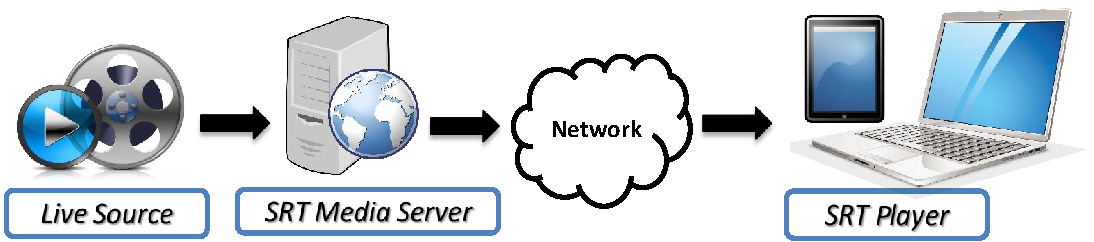
\includegraphics[width=1\textwidth,keepaspectratio]{scenario.pdf}
	\caption{System architecture for SRT streaming.}
	\label{fig:BMSB2020system}
\end{figure}

The system architecture for delivering SRT streams is depicted in Figure \ref{fig:BMSB2020system}. The system is composed by a Live Source, a SRT Media Server and a SRT Player.

The Live Source is the node which provides the content to the processing and delivery pipeline. Here, many different entities can act as a Live source, e.g. a camera or a video software editor.

The SRT Media Server processes the content ingested by the Live Source and delivers it to the SRT Player after encoding and packetizing it into an SRT-compliant stream. Thus, it accomplishes the following tasks:
\begin{itemize}
	\item Encoding: it encodes the content into a live H.264 bitstream \cite{wiegand2003}. In a legacy SRT solution, the video frame resolution and encoding bitrate is chosen when launching the encoding process and kept unaltered during all the process. In our approach, both resolution and bitrate can be dynamically changed during the streaming session to provide different representation levels of the same content.
	\item Muxing: H.264 bitstream is packetized into a MPEG-2 Transport Stream (MPEG-TS) container \cite{sarginson1996}.
	\item Encryption: MPEG-TS is encrypted though 128/256 bit Advanced Encryption Standard (AES) \cite{chown2002advanced}. This is a mandatory feature included in SRT to enforce end-to-end security.
	\item Delivery: SRT employs User Datagram Protocol (UDP) to transmit data over the network to the client since it guarantees lower latency than Transmission Control Protocol (TCP), which is commonly used by HTTP-based streaming solutions. However, UDP is not reliable since it does not provide mechanisms to compensate for transmission errors. Then, SRT includes Forward Error Correction (FEC) and re-transmission mechanisms on top of UDP delivery to allow the SRT Player to recover from lost or corrupted packets.
	\item Monitoring: SRT server receives network reports from the SRT Player which contain information related to network status (bandwidth and delay) and packet transmission (sent, lost or re-transmitted packets number). In a legacy SRT solution, reports are only employed to tune the sending transmission rate and schedule the transmission of new and/or lost packets. In our approach, network reports are also captured and employed to select the appropriate representation level (resolution and bitrate) to be used by the encoding process.
\end{itemize}

We employ GStreamer \cite{gstreamer} in its v1.14 stable release to develop our Adaptive Rate Control-enabled SRT Media server. We select and setup the following plugins to accomplish the above tasks:

\begin{itemize}
	\item \textit{H.264 encoder}: the setup of the encoder is key to allow the adaptation of the representation (resolution and bitrate) of the content according to the measured network statistics. \textit{Keyframes} (I-frames) do not require any other frames to be decoded, so the player can always start decoding a stream from a \textit{keyframe}. Thus, \textit{keyframes} are essential for live streaming to start playing the content as soon as possible when the player starts receiving the content. Moreover, in our Adaptive Rate Control-enabled stream, when it switches the representation level, it introduces a discontinuity. Thus, it makes new frames, with a different resolution and encoding bitrate, not possible to be decoded based on the previous frames. The player needs a new \textit{keyframe} to decode the stream every time the representation level changes. Then, the Adaptive Rate Control forces the encoder to introduce a \textit{keyframe} every time a representation switch is performed.
	\item \textit{MPEG-TS muxer}: it packetizes H.264 encoded frames into MPEG-TS chunks. Each chunk cannot contain data at different representation levels. Then, it is mandatory that each MPEG-TS chunk starts with a \textit{keyframe}.
	\item \textit{SRT server sink}: it receives MPEG-TS chunks from the muxer, it encrypts and encapsulates them into UDP packets before sending them to the player. This plugin gets active, sending packets, only when a client is connected.
	It also monitors the network by getting network statistics measured during the transmission of the video stream to the client. A legacy SRT server sink uses statistics only to adapt the network overhead of the transmission, to reduce packets lost and to avoid re-transmissions. Additionally, the proposed Adaptive Rate Control-enabled solution exploits this information to dynamically change the setup of the encoder plugin to switch to a suitable representation level.
\end{itemize}

Finally, SRT player is implemented with GStreamer release (v1.14) \cite{gstreamer}. This version provides SRT client and decoding capabilities. Thus, it can play SRT legacy streams. Moreover, the aggregation of the Adaptive Rate Control to the SRT Media server does not cause any relevant change in the protocol. This means that developing a custom client application is not required and the generated SRT stream can be played by any SRT-compliant player.

\begin{figure}[htp]
	\centering 
	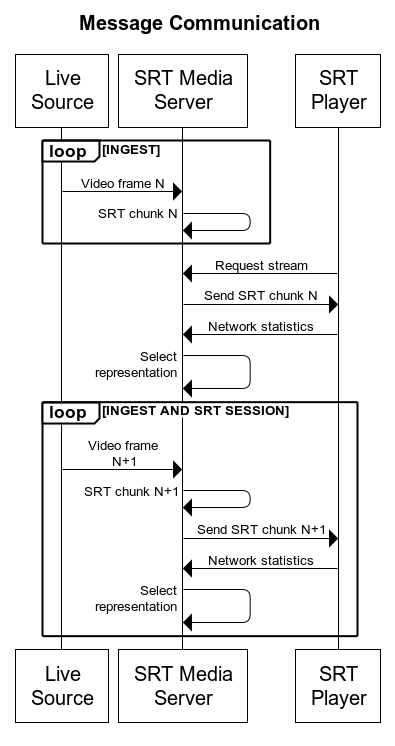
\includegraphics[width=0.6\textwidth,keepaspectratio]{webseq.png}
	\caption{Sequence diagram.}
	\label{fig:BMSB2020sequence}
\end{figure}

The communication between the systems in the setup is shown in Figure \ref{fig:BMSB2020sequence}. SRT Media Server starts to encode and packetize video frames when the Live Source is connected. Video frames are H.264 encoded and MPEG-TS muxed, then packetized into SRT chunks.
Nevertheless, data are not transmitted until an SRT player connects to the SRT Media Server. It means that chunks can be discarded by the server if there are no players. The SRT Media Server only stores the most recent chunks with a buffer size of "maximum allowed latency". This operation is necessary in order to guarantee that only the most recent chunks are sent, then achieve a low latency live streaming. In GStreamer, maximum allowed latency is configurable, but we decide to keep it to its default value which is 125 ms. Once the SRT player is connected, SRT Media Server starts delivering the content to the player. While receiving the content, the SRT player stores it in the playback buffer before decoding and displaying it. The playback buffer is set to 1 seconds to balance low latency, packet losses reliability and changeable network conditions.

To adapt the representation, the implemented Adaptive Rate Control accesses network statistics from the SRT server sink plugin and exploits the information to tune the configuration of the H.264 encoder. This evaluation is performed by the Adaptive Rate Control once per second. The decision algorithm of the implemented Adaptive Rate Control is shown in Algorithm \ref{alg:BMSB2020algorithm}. The algorithm takes the last measured network bandwidth (\textit{bw$_t$}), round-trip delay time (\textit{rtt$_t$}) and send rate (\textit{rate$_t$}) from SRT network reports, the current employed representation level (\textit{rep$_t$}) and the list of all the available ones (\textit{\{rep$_{list}$\}}). Bandwidth and round-trip delay time are employed to evaluate the maximum allowed network throughput (\textit{throughput$_{max_t}$}) through the Equation \ref{eq:BMSB2020thoughput}.

\begin{algorithm}
	\renewcommand{\algorithmicrequire}{\textbf{Input:}}
	\renewcommand{\algorithmicensure}{\textbf{Output:}}
	\caption{Adaptive Rate Control}
	\label{alg:BMSB2020algorithm}
	\begin{algorithmic}
		\Function{adaptiveRate}{bw$_{t}$, rtt$_{t}$, rate$_{t}$, rep$_{t}$, $\{rep_{list}\}$}
		\Require bw$_t$ \Comment{measured bandwidth}
		\Require rtt$_t$ \Comment{measured delay}
		\Require rate$_t$ \Comment{measured send rate}
		\Require rep$_t$ \Comment{current representation}
		\Require $\{rep_{list}\}$ \Comment{available representations}
		\Ensure rep$_{t+1}$ \Comment{next representation}
		\State throughput$_{max_t}$ $\leftarrow$ bw$_{t}$, rtt$_{t}$ \Comment{network throughput}
		\ForAll { rep$^{i}$ $\in$ $\{rep_{list}\}$ } \Comment{for each representation}
		\State bitrate$^{i}_{t}$ $\leftarrow$ rep$^{i}$, rate$_{t}$, rep$_t$ \Comment{\parbox[t]{0.31\linewidth}{minimum network bitrate}}
		\If {(throughput$_{max_t}$ $>$ throughput$^{i}_{t}$)} %\Comment{\parbox[t]{0.1\linewidth}{network admits the bitrate}}
		\State \Comment{network admits the representation}
		\State rep$_{t+1}$ $\leftarrow$ rep$^i$ \Comment{next representation}
		\EndIf
		\EndFor
		\EndFunction
	\end{algorithmic}
\end{algorithm}

\begin{equation}
\label{eq:BMSB2020thoughput}
throughput_{max_t} = bw_t * \frac{1}{1 + \frac{rtt_t}{2}}
\end{equation}

Then, for each available representation, the required network throughput to allow its transmission is calculated. It is important to note that each representation means a different throughput configured by the encoding bitrate. Furthermore, the encoding bitrate needs to accommodate a gap to allow that protocols messages and extra information from other levels of the ISO/OSI model, added to the encoded video payloads, still meet network bandwidth thresholds.

Consequently, to establish if it is possible to stream a specific representation to the client, we should compare the maximum allowed network throughput (\textit{throughput$_{max_t}$}) with the throughput that the representation would generate (\textit{throughput$^i_t$}). Since we cannot access the employed throughput before streaming the content, we estimate it from the current send rate (\textit{rate$_t$}) provided by the network reports. Equation \ref{eq:BMSB2020minBW} estimates the necessary network throughput (\textit{throughput$_t^i$}) to allow the representation (\textit{rep$^i$}) bitrate to be streamed. The ratio between current send rate (\textit{rate$_t$}) and current representation encoding bitrate (\textit{rep$_t$}) is the current overhead, then we multiply it per the representation encoding bitrate (\textit{rep$^i$}).

\begin{equation}
\label{eq:BMSB2020minBW}
%bitrate^{i}_{t} = rep^i * \frac{rate_{t}}{rep_{t}}
throughput^{i}_{t} = rep^i * \frac{rate_{t}}{rep_{t}}
\end{equation}

If the estimated throughput (\textit{throughput$_t^i$}) is lower than the maximum allowed throughput (\textit{throughput$_{max_t}$}), it means that the representation can be sent. The output of the algorithm is the selected representation to be employed at the H.264 encoder. The encoder is configured to immediately generate a \textit{keyframe} and switch at the new selected representation resolution and encoding bitrate.

\subsection{Results}
\label{sec:BMSB2020results}

The experimental setup employed for testing the implemented Adaptive Rate Control is presented in Figure \ref{fig:BMSB2020setup}. The overall setup comprises the following nodes:
\begin{itemize}
	\item STR Media Server and Traffic Control: this is a unique physical node which embeds two logical systems. We employ a Docker containerization \cite{merkel2014} to run different functions in separated environments. A Docker container running Ubuntu 19.04 OS includes the Adaptive Rate Control-enabled SRT Media Server developed through GStreamer framework \cite{gstreamer}. The container communicates with the host machine running Ubuntu 16.04 OS which forwards data to the physical network interface. On the host machine, we periodically modify bandwidth and latency of the network interface. Traffic Control \cite{tc} is the utility to change the uplink capacity. To emulate an LTE network, we use the \textit{European Broadband user experience} dataset collected and publicly provided by the Joint Research Centre (JCR) of the European Commission \cite{chawdhry2016}. The dataset provides both bandwidth and latency that we apply through Traffic Control utility. The interval between two consecutive network changes is set to 100 ms. %, aligned with the dataset sample rate.
	\item Network switch: this node provides wired network access to both server and player nodes to communicate each other. It forwards all the incoming traffic on both sides.
	\item SRT Player: this node run a GStreamer application to receive the SRT stream and play it.
\end{itemize}

\begin{figure}[htp]
	\centering
	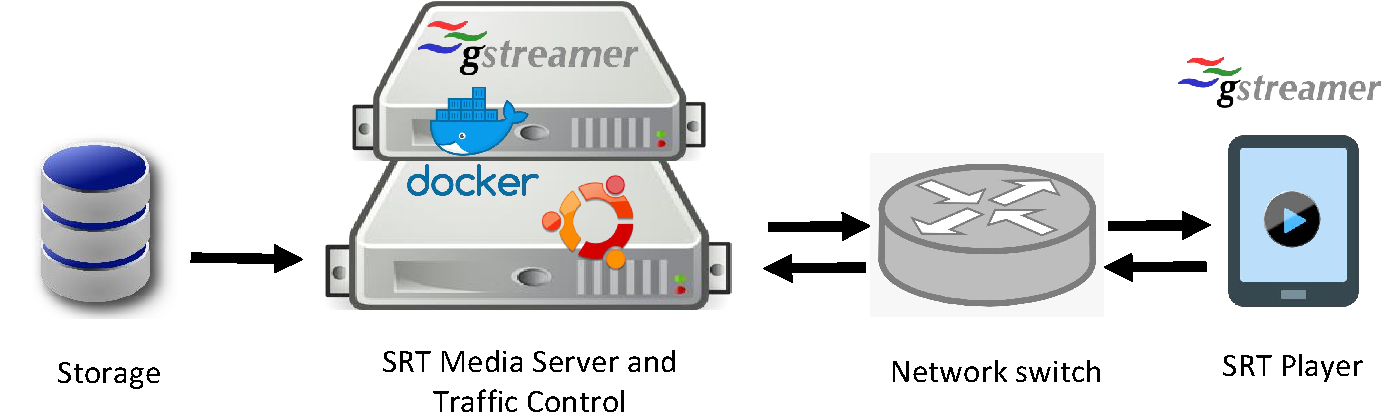
\includegraphics[width=1\textwidth,keepaspectratio]{testbed.pdf}
	\caption{Experimental setup.}
	\label{fig:BMSB2020setup}
\end{figure}

\begin{table}[htp]
	\caption{Set of representations employed in the experiments.}
	\centering
	\bgroup
	\def\arraystretch{1.2}%  1 is the default, change whatever you need
	\setlength\tabcolsep{2.5pt} % default value: 6pt
	\label{tab:BMSB2020reps}
	{\scriptsize
		\begin{tabular}{>{\centering\arraybackslash}m{\dimexpr0.1\textwidth-2\tabcolsep-\arrayrulewidth\relax}
				>{\centering\arraybackslash}m{\dimexpr0.15\textwidth-2\tabcolsep-\arrayrulewidth\relax}
				>{\centering\arraybackslash}m{\dimexpr0.15\textwidth-2\tabcolsep-\arrayrulewidth\relax}
				>{\centering\arraybackslash}m{\dimexpr0.15\textwidth-2\tabcolsep-\arrayrulewidth\relax}
			}
			\toprule
			\textbf{Index} & \textbf{bitrate (kbps)} & \textbf{resolution} & \textbf{framerate (FPS)} \\
			\midrule
			\midrule
			1 & 1200 & 640x360 & 24 \\
			2 & 2250 & 1280x720 & 24 \\
			3 & 4500 & 1920x1080 & 24 \\
			\bottomrule
			\bottomrule
		\end{tabular}
		\egroup
	}
\end{table}

We perform different experiments to compare the Adaptive Rate Control-enable SRT stream with a legacy SRT stream. We use a locally stored Big Buck Bunny test sequence to feed the SRT Media Server. Its raw version is provided by Xiph.Org Foundation \cite{xiph}. For the Adaptive Rate Control-enabled stream, we established three different representation levels to be employed by the H.264 encoder, while legacy one employs only the higher one. The representations are shown in Table \ref{tab:BMSB2020reps}.

The duration of each SRT streaming session lasts 594 seconds which is the duration of the employed test sequence. The results of the two strategies in terms of representation switches, freezes, initial delay and average representation bitrate are shown in Table \ref{tab:BMSB2020results}.

\begin{table}[htp]
	\caption{Number of switches (\textit{S$_{Nb}$}), number of freezes (\textit{F$_{Nb}$}), average freeze duration (\textit{F$_{avg}$}), initial delay (\textit{D}) and average representation bitrate (\textit{R$_{avg}$}) for both legacy and Adaptive Rate Control-enabled SRT streams.}
	\centering
	\def\arraystretch{1.2}%  1 is the default, change whatever you need
	\setlength\tabcolsep{2.5pt} % default value: 6pt
	\label{tab:BMSB2020results}
	{\scriptsize
		\begin{tabular}{>{\centering\arraybackslash}m{\dimexpr0.2\textwidth-2\tabcolsep-\arrayrulewidth\relax}
			>{\centering\arraybackslash}m{\dimexpr0.1\textwidth-2\tabcolsep-\arrayrulewidth\relax}
			>{\centering\arraybackslash}m{\dimexpr0.1\textwidth-2\tabcolsep-\arrayrulewidth\relax}
			>{\centering\arraybackslash}m{\dimexpr0.1\textwidth-2\tabcolsep-\arrayrulewidth\relax}
			>{\centering\arraybackslash}m{\dimexpr0.1\textwidth-2\tabcolsep-\arrayrulewidth\relax}
			>{\centering\arraybackslash}m{\dimexpr0.1\textwidth-2\tabcolsep-\arrayrulewidth\relax}
		}
		\toprule
		\textbf{SRT server} & \textbf{S$_{\textbf{Nb}}$} & \textbf{F$_{\textbf{Nb}}$} & \textbf{F$_{\textbf{avg}}$(ms)} & \textbf{D(ms)} & \textbf{R$_{\textbf{avg}}$(kbps)}\\
		\midrule
		\midrule
		Legacy & 0 & 122 & 820 & 972 & 4500 \\
		Adaptive Rate Control & 197 & 87 & 727 & 986 & 4028 \\
		\bottomrule
		\bottomrule
	\end{tabular}
	}
\end{table}

\begin{figure}[htp]
	\centering 
	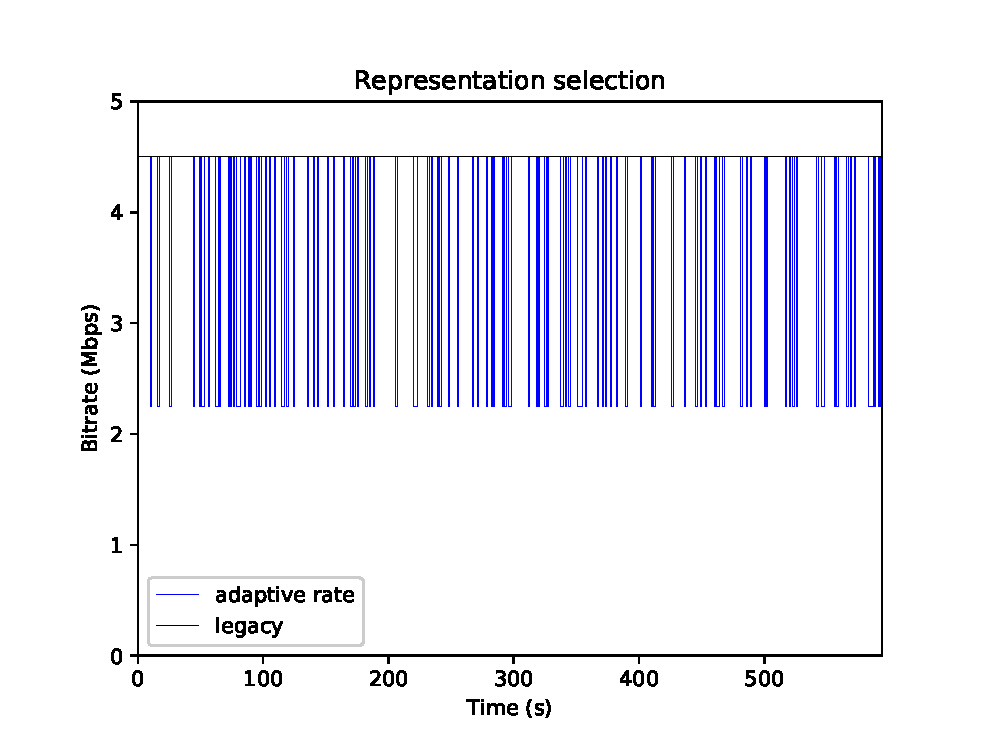
\includegraphics[width=1\textwidth,keepaspectratio]{reps.eps}
	\caption{Representation bitrate selection.}
	\label{fig:BMSB2020selection}
\end{figure}

In terms of switches, Adaptive Rate Control solution performs 197 representation switches, while it is not applicable to the legacy SRT stream. Figure \ref{fig:BMSB2020selection} shows the distribution of the switches across the streaming session. Legacy stream is stable to 4500 kbps encoding bitrate, while seems that Adaptive Rate Control one never uses the lowest encoding bitrate (1200 kbps) but moves between the other two (4500 and 2250 kbps). Thus, it causes that the average representation bitrate is 10\% lower when using the Adaptive Rate Control (4028 kbps against 4500 kbps). In terms of initial delay, there is not a noticeable difference since the Adaptive Rate Control does not introduce any delay while starting the streaming session. On the contrary, our Adaptive Rate Control solution outperforms legacy one while considering number of freezes and their duration. Here, the proposed solution scores 29\% less freezes events, and their average duration is 11\% shorter.

These results show that our solution sacrifices average representation bitrate in order to reduce freezes events. Fewer freezes events lead to a smoother video playback for the end user.

\subsection{Conclusions and Future Work}
\label{sec:BMSB2020conlusion}
This paper proposes an Adaptive Rate Control for SRT protocol to deliver live streaming content, while coping with transmission variability due to network degradation or issues.

The proposed solution is integrated with Open Source GStreamer multimedia framework and tested by altering the network capabilities according to real LTE measurements provided by a publicly available dataset.

Compared to a legacy SRT solution, the results show that Adaptive Rate Control-enabled SRT delivery experiences fewer freeze events by enabling switching operations to lower representation bitrates. Thus, it reduces the average representation bitrate to prioritize playback smoothness.


% use section* for acknowledgement
%\subsection*{Acknowledgment}